\documentclass[journal]{IEEEtran}

% Packages
\usepackage{cite}
\usepackage{graphicx}
\usepackage{subfigure}
\usepackage{float}
\usepackage{url}
\usepackage{color}
\usepackage{amsmath}


\begin{document}

% paper title
% can use linebreaks \\ within to get better formatting as desired
\title{Visual~Perception~Lab~2 \\ Camera~Calibration}
%

\author{Rodrigo~Caye~Daudt}

\definecolor{lightgray}{gray}{0.5}



% make the title area
\maketitle



%%%%%%%%%%%%%%%%%%%%%%%%%%%%%%%%%%%%%%%%%%%%%%%%%%%%%%%%%%%%%%%%%%%%%%%%%%%%%%%
\section{Introduction}

\IEEEPARstart{T}{his} report describes the work done for lab session 2 on the Visual Perception class. The main focus of this work was to better understand the mathematical operations that model a pinhole camera, as well as the camera calibration methods of Hall and Faugeras (without distortion).

%%%%%%%%%%%%%%%%%%%%%%%%%%%%%%%%%%%%%%%%%%%%%%%%%%%%%%%%%%%%%%%%%%%%%%%%%%%%%%%
\section{Part 1}\label{p1}

\subsection{Step 1}

The first step was simply to define the intrinsic and extrinsic parameters of the camera. The intrinsic parameters are the ones that describe the workings of the camera, while the extrinsic parameters define the position of the camera relative to the world. The used parameters are included in Tables \ref{intrinsics} and \ref{extrinsics}. The camera sensor was assumed to have size $640\times 480$.

\begin{table}[H]
	\caption{Intrinsic parameters}
	\centering
	\begin{tabular}{l | r r r r r}\label{intrinsics}
		Parameter & au & av & u0 & v0 & f\\
		\hline
		Value & 557.0943 & 712.9824 & 326.3819 & 298.6679 & 80\\
	\end{tabular}
\end{table}

\begin{table}[H]
	\caption{Extrinsic parameters}
	\centering
	\begin{tabular}{l | r r r r r r}\label{extrinsics}
		Parameter & Tx & Ty & Tz & Phix & Phiy & Phix1\\
		\hline
		Value & 100 & 0 & 1500 & $0.4\pi$ & $-0.9\pi$ & $\pi /5$\\
	\end{tabular}
\end{table}

\subsection{Step 2}

The next step was to compute the intrinsic and extrinsic transformation matrices based on the parameters set on step 1.The matrix forms and operations used to calculate these matrices based on the parameters are shown below. It is important to remark that the matrix $T$ was normalised by the element $T(3,4)$ to facilitate comparisons with the results from the camera calibration calculations.

\[
T_{int} = 
\begin{bmatrix}
    \alpha_u & 0 & u_0 & 0 \\
    0 & \alpha_v & v_0 & 0 \\
    0 & 0 & 1 & 0
\end{bmatrix}
\]

\[
R_x(\Phi) = 
\begin{bmatrix}
    1 & 0 & 0 \\
    0 & cos(\Phi) & -sin(\Phi) \\
    0 & sin(\Phi) & cos(\Phi)
\end{bmatrix}
\]

\[
R_y(\Phi) = 
\begin{bmatrix}
    cos(\Phi) & 0 & sin(\Phi) \\
    0 & 1 & 0 \\
    -sin(\Phi) & 0 & cos(\Phi)
\end{bmatrix}
\]

\[
R = R_x(Phix) \times R_y(Phiy) \times R_x(Phix1)
\]

\[
trans = 
\begin{bmatrix}
    T_x & T_y & T_z 
\end{bmatrix}^T
\]

\[
T_{ext} = 
\begin{bmatrix}
    R & trans \\
    0_{1 \times 3} & 1
\end{bmatrix}
\]

\[
T = T_{int} \times T_{ext}
\]

\subsection{Step 3}

In this step, six points were generated at random positions, with world coordinates $x$, $y$, and $z$  in the range $[-480,480]$. Six points were used since that is the minimum amount of points possible to perform camera calibration. These points were used on the following steps as example points for calculating projections and calibrating the camera. It is important to note that since these points were generated randomly each time the program was executed, the results obtained in the following steps varied slightly between different runs.

\subsection{Step 4}

On this step, the objective was to calculate the projection of the points into the camera sensor. The camera sensor coordinates were calculated using the following equation, which uses the matrices calculated in step 2:

\[
projections = T \times points
\]

The calculated points were then adjusted so that their scales (value of $s$) was 1 so that the projected points could be correctly plotted.

\subsection{Step 5}

Step 5 consisted simply on plotting the point projections using the pixel coordinates. Figure \ref{projections} shows the result of this plotting one time the program was run. The projection points are displayed in blue, while the sensor borders are showed in red. 

It was observed that some not all points were inside the sensor boundaries on every run, which would be a problem for real cameras, but since our camera was simulated we could work with coordinate values outside the boundaries of the sensor. It is also important to note that more well spread points would usually lead to better precision when calibrating the camera.

\begin{figure}[H]
	\centering
	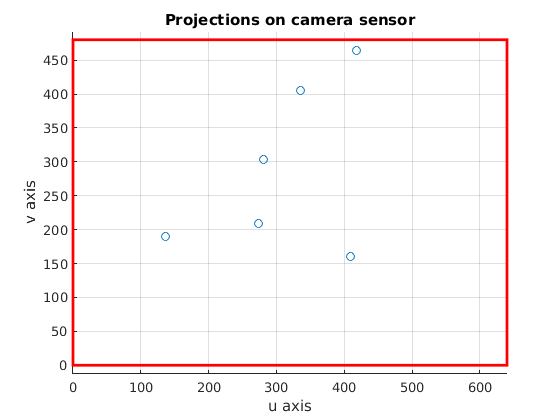
\includegraphics[width=0.8\linewidth]{figures/projections.png}
	\caption{Point projections onto camera sensor}
	\label{projections}
\end{figure}


\subsection{Step 6}

On this step an estimation of the transformation matrix $T$ was calculated using the method of Hall. A function \textit{hall\_cc} that performs camera calibration using the Hall method was written since it was used in several of the following sections and for eventual use in the future. This function takes as input only the coordinates in the world coordinate system and their projections' coordinates. The output of this function is the matrix $A$, which is an estimation of the pure projection matrix $T$. The code for the function that was used for computing the matrix $A$ using the method of Hall is found in Appendix \ref{hall}.

\subsection{Step 7}

To evaluate the results obtained in step 6 we compared the calculated the ratio between the elements of the calculated matrix $A$ and their respective values in $T$ using the MATLAB command $$ratio\_pure = A\_hall./T$$, which divided each element of $A\_hall$ with the element in the same position in $T$. As expected, the result was

\[
ratio\_hall = 
\begin{bmatrix}
    1 & 1 & 1 & 1 \\
    1 & 1 & 1 & 1 \\
    1 & 1 & 1 & 1 
\end{bmatrix}
\]

which means all values in $A$ were exactly the same as the values in $T$. This result is so good since there was no added noise in any of the coordinate values used for camera calibration.

\subsection{Step 8}

The objective of step 8 was to evaluate the robustness of the camera calibration method of Hall regarding to noise. Gaussian noise in the range $[-1;1]$ was added to 95\% of the projection points used in step 6 and then the method of Hall was applied using the noisy projections.

To evaluate the results, the calculated matrix was used to recompute the projections of the points and the mean distance between the correct projections and the distorted projections was calculated. In one example case, the calculated mean distance was $2.3781$. Also, the same element-by-element ratio used in step 7 was used and the found result was the following:

\[
ratio\_noisy6 = 
\begin{bmatrix}
    1.0002  &  0.9993  &  0.9892  &  0.9982 \\
    0.9906  &  1.0060  &  0.9506  &  0.9965 \\
    0.9834  &  1.0264  &  1.0090  &  1.0000 
\end{bmatrix}
\]

This results clearly show that the calculated parameters varied slightly from the true parameters, and that the added noise had an impact on the precision of the calculation of $A$.

Figure \ref{noisycc} shows  an example of such projections plotted on the same image. Figure \ref{noisycczoom} shows the detailed image of the projections of a given point, and it is easy to observe a distance of roughly 1 pixel between these two projection points.

\begin{figure}[H]
	\centering

	\subfigure[Correct projections (blue) along projections calculated with noisy A matrix (red)]{\label{noisycc}
		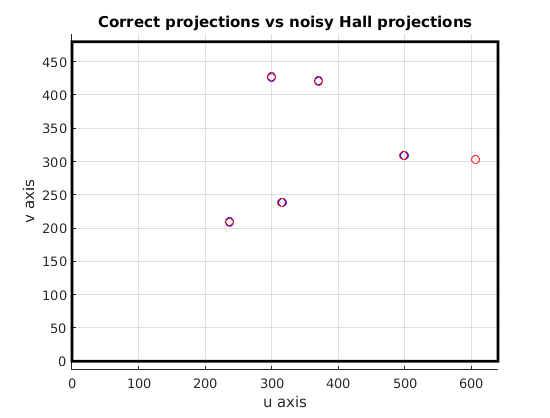
\includegraphics[width=0.8\linewidth]{figures/noisycc.png}}\\
	\subfigure[Zoom on a pixel shows the difference in position between projection calculated with T or A matrices]{\label{noisycczoom}
		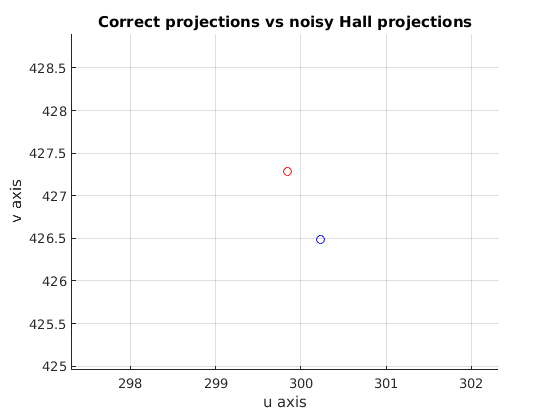
\includegraphics[width=0.8\linewidth]{figures/noisycczoom.png}}
	\caption{Representation of correct and noisy projections onto camera sensor}
	\label{fig:noisycc}
\end{figure}



\subsection{Step 9}

In step 9 the steps of step 8 were repeated when using more points and the same amount of noise to evaluate how the usage of more points helps with the robustness of the calculated results. The process was repeated using 6, 10, 50 and 200 points. The mean distance between the correct projections and the projections calculated with the computed $A$ matrix are shown in Table \ref{hakuna} below.

\begin{table}[H]
	\caption{Precision of A for various amounts of points}
	\centering
	\begin{tabular}{l | r r r r}\label{hakuna}
		Number of points & 6 & 10 & 50 & 200 \\
		\hline
		Mean distance & 2.3781 & 2.0876 & 1.5357 & 1.3310 \\
	\end{tabular}
\end{table}

It is easy to see that the usage of more points make the result more precise, but even using 200 points our mean distance was still at 1.3310. This may or may not be a problem depending on the application for which the camera calibration is necessary. Also, the calculations made here do not take into account any kind of distortion, which may be present in real cameras, and that would further decrease the precision of our approximation.

%%%%%%%%%%%%%%%%%%%%%%%%%%%%%%%%%%%%%%%%%%%%%%%%%%%%%%%%%%%%%%%%%%%%%%%%%%%%%%%
\section{Part 2}\label{p2}\definecolor{lightgray}{gray}{0.5}


\subsection{Step 10}

The objective in step 10 was to perform camera calibration using the Faugeras method. Unlike the method of Hall, which tries to approximate $T$ directly, the Faugeras method calculates a vector $X$ which allows us to calculate T as well as calculating the intrinsic and extrinsic parameters for the camera. For the same reasons as in the method of Hall, a function \textit{faugeras\_cc} was written to perform the Faugeras camera calibration calculations. Other functions were also written to calculate the intrinsic parameters, the extrinsic parameters, and the matrix $A$ from the calculated $X$ vector.

As was to be expected, the ratio between the $A$ estimation of $T$ using the Faugeras method with no added noise was:

\[
ratio\_faugeras = 
\begin{bmatrix}
    1 & 1 & 1 & 1 \\
    1 & 1 & 1 & 1 \\
    1 & 1 & 1 & 1 
\end{bmatrix}
\]

The differences between the original and the calculated intrinsic and extrinsic parameters were calculated. The largest of these errors was of the order of $10^{-11}$, which we can attribute to numerical error from the mathematical operations performed by MATLAB.


\subsection{Step 11}

In step 11 step 10 was repeated with different levels of noise, i.e. noise in ranges $[-1;1]$, $[-2;2]$, or $[-3;3]$ was applied to 95\% of the points. Once again the difference between the correct parameters and the estimated parameters was calculated. The results of one given run are shown in Table \ref{matata}.

\begin{table}[H]
	\caption{Difference between original and calculated parameters}
	\centering
	\begin{tabular}{l | r r r}\label{matata}
		Measurement & $[-1;1]$ & $[-2;2]$ & $[-3;3]$ \\
		\hline
		au & -58.4496 & 3.5019 & 153.1380 \\
		u0 & -20.3580 & 89.6070 & 82.2640 \\
		av & -71.7524 & 9.2393 & 186.5883 \\
		v0 & 17.8783 & -71.8777 & -93.6513 \\
		translation & 174.1966 & 274.7029 & 502.8571 \\
	\end{tabular}
\end{table}

It was observed that these results varied a lot between runs. We can observe from the values in Table \ref{matata} that the estimation of intrinsic and extrinsic parameters was not very precise when using points with added noise. On the other hand, it is also easy to see that the error in the calculated parameters tended to increase when more noise was added, which was expected.

To compare the precision of the methods of Hall and Faugeras for camera calibration, the mean distances between the projection points using each method were calculated. These values can me found in Table \ref{noworries}.

\begin{table}[H]
	\caption{Difference in precision between Hall and Faugeras camera calibration methods}
	\centering
	\begin{tabular}{l | r r r}\label{noworries}
		Measurement & $[-1;1]$ & $[-2;2]$ & $[-3;3]$ \\
		\hline
		Hall & 1.5044 & 2.2849 & 3.3045 \\
		Faugeras & 1.5044 & 2.2849 & 3.3045 \\
	\end{tabular}
\end{table}


These values suggest that both calculations have the same precision when estimating the projections. One possible explanation for this phenomenon is that both methods achieve the best possible result for $A$ given a set of points and projections since both are deterministic methods.

Finally, one possible explanation for the high variability and error in the calculated values for the parameters was that the Faugeras method did everything possible to calculate $A$ as precisely as possible, and this resulted in bending the estimated intrinsic and extrinsic parameters' estimations a fair amount.

%%%%%%%%%%%%%%%%%%%%%%%%%%%%%%%%%%%%%%%%%%%%%%%%%%%%%%%%%%%%%%%%%%%%%%%%%%%%%%%
\section{Part 3}\label{p3}

\subsection{Step 12}

The last step of this lab assignment was to plot in one image the whole scene. This included the camera center, the camera coordinate system, the camera sensor, the random points, the projection rays, and the projected points. The scene representation is shown in Fig. \ref{scene}. We can see the projection rays converge on the camera center. We can also see in Fig. \ref{scenezoom} that the projections of the points onto the camera sensor are all positioned on the intersections of the projection rays and the camera sensor.


\begin{figure}[p]
	\centering

	\subfigure[]{\label{scene}
		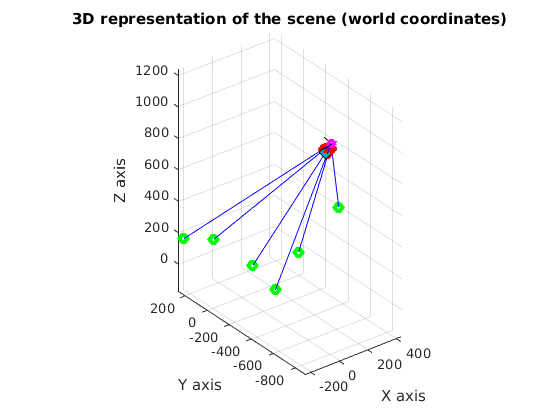
\includegraphics[width=0.8\linewidth]{figures/scene.png}}\\
	\subfigure[]{\label{scenezoom}
		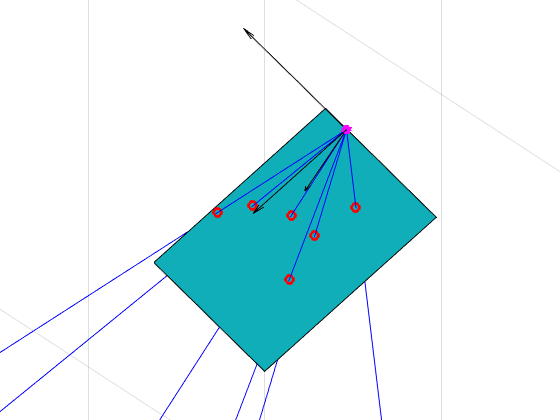
\includegraphics[width=0.8\linewidth]{figures/scenezoom.png}}
	\caption{3D scene representation}
	\label{fig:scene}
\end{figure}





%%%%%%%%%%%%%%%%%%%%%%%%%%%%%%%%%%%%%%%%%%%%%%%%%%%%%%%%%%%%%%%%%%%%%%%%%%%%%%%
\section{Conclusion}\label{conclusion}

This report described all the work done relative to the lab session 2, which focused on the camera calibration methods of Hall and Faugeras without distortion. This procedure was very helpful in the learning process of these methods, along with solidifying the knowledge of rigid bodies transformation. It was very interesting and enlightening to implement both camera calibration methods, and to observe their responses to different amounts of points and noise levels. Finally, part 12 was very helpful with fully understanding how homogeneous coordinates work and how to use it.

All the MATLAB code that was developed for this work will be provided along this report for evaluation. The main file that should be executed to obtain the described results is \textit{lab2\_script.m}.


\appendices

%%%%%%%%%%%%%%%%%%%%%%%%%%%%%%%%%%%%%%%%%%%%%%%%%%%%%%%%%%%%%%%%%%%%%%%%%%%%%%%
\begin{figure*}[p]
\section{hall\_cc.m}\label{hall}
    \begin{verbatim}
function A_hall= hall_cc(points,projections_sc)
% Camera calibration using Hall method
%   points - 4xN matrix with real word coordinates of points
%   projections - 3xN matrix with scaled projections
%   A_hall - output projection matrix
% Daudt - 19/03/16

num_points = size(points,2);

assert(size(points,1) == 4);
assert(num_points >= 6);
assert(size(projections_sc,2) == num_points);

if min(projections_sc(3,:)) ~= 1 || max(projections_sc(3,:)) ~= 1
    for i = 1:3
        projections_sc(i,:) = projections_sc(i,:)./projections_sc(3,:);
    end
end

Q = zeros(2*num_points,11);
B = zeros(2*num_points,1);
for i = 1:num_points
    IXui = projections_sc(1,i);
    IYui = projections_sc(2,i);
    Q(2*i-1,:) = [points(1,i) points(2,i) points(3,i) 1 0 0 0 0 
                  -IXui*points(1,i) -IXui*points(2,i) -IXui*points(3,i)];
    Q(2*i,:) = [0 0 0 0 points(1,i) points(2,i) points(3,i) 1 
                  -IYui*points(1,i) -IYui*points(2,i) -IYui*points(3,i)];
    B(2*i-1) = projections_sc(1,i);
    B(2*i) = projections_sc(2,i);
end
A = Q\B;
A_hall = [A(1) A(2) A(3) A(4);A(5) A(6) A(7) A(8);A(9) A(10) A(11) 1];

end
\end{verbatim}
\end{figure*}

%%%%%%%%%%%%%%%%%%%%%%%%%%%%%%%%%%%%%%%%%%%%%%%%%%%%%%%%%%%%%%%%%%%%%%%%%%%%%%%
\begin{figure*}[p]
\section{faugeras\_cc.m}\label{faugeras}
\begin{verbatim}
function X = faugeras_cc(points,projections_sc)
% Camera calibration using Faugeras method
%   points - 4xN matrix with real word coordinates of points
%   projections - 3xN matrix with scaled projections
%   X - output X vector
% Daudt - 19/03/16

num_points = size(points,2);

assert(size(points,1) == 4);
assert(num_points >= 6);
assert(size(projections_sc,2) == num_points);

if min(projections_sc(3,:)) ~= 1 || max(projections_sc(3,:)) ~= 1
    for i = 1:3
        projections_sc(i,:) = projections_sc(i,:)./projections_sc(3,:);
    end
end

Q = zeros(2*num_points,11);
B = zeros(2*num_points,1);
for i = 1:num_points
    Q(2*i-1,:) = [points(1:3,i)' (-projections_sc(1,i)*points(1:3,i)') 0 0 0 1 0];
    Q(2*i,:) = [0 0 0 (-projections_sc(2,i)*points(1:3,i)') points(1:3,i)' 0 1];
    B(2*i-1) = projections_sc(1,i);
    B(2*i) = projections_sc(2,i);
end

X = Q\B;

end
\end{verbatim}
\end{figure*}

%\bibliographystyle{IEEEtran}
%\bibliography{Template_Daudt}


\end{document}


